\documentclass[a4paper,12pt]{article}
\usepackage[utf8]{inputenc}
\usepackage[spanish]{babel}
\usepackage{color}
\usepackage{parskip}
\usepackage{graphicx}
\usepackage{multirow}
\usepackage{listings}
\usepackage{vmargin}
\usepackage{datetime}
\newdate{date}{9}{11}{2017}
\graphicspath{ {imagenes/} }
\definecolor{mygreen}{rgb}{0,0.6,0}
\definecolor{lbcolor}{rgb}{0.9,0.9,0.9}
\usepackage{epstopdf}
\usepackage{float}


\setpapersize{A4}
\setmargins{2.5cm}       % margen izquierdo
{1.5cm}                        % margen superior
{16.5cm}                      % anchura del texto
{23.42cm}                    % altura del texto
{10pt}                           % altura de los encabezados
{1cm}                           % espacio entre el texto y los encabezados
{0pt}                             % altura del pie de página
{2cm}     

\lstset{
    tabsize=4,    
%   rulecolor=,
    language=[GNU]C++,
        basicstyle=\tiny,
        aboveskip={1.5\baselineskip},
        columns=fixed,
        showstringspaces=false,
        extendedchars=false,
        breaklines=true,
        prebreak = \raisebox{0ex}[0ex][0ex]{\ensuremath{\hookleftarrow}},
        frame=single,
        showtabs=false,
        showspaces=false,
        showstringspaces=false,
        identifierstyle=\ttfamily,
        keywordstyle=\color[rgb]{0,0,1},
        commentstyle=\color[rgb]{0.026,0.112,0.095},
        numberstyle=\color[rgb]{0.205, 0.142, 0.73},
%        \lstdefinestyle{C++}{language=C++,style=numbers}’.
}


\begin{document}
\title{Analisador léxico con Flex}
\author{
Christofer Fabián Chávez Carazas \\
\small{Universidad Nacional de San Agustín de Arequipa} \\
\small{Escuela Profesional de Ciencia de la Computación} \\
\small{Compiladores}
}
\date{\displaydate{date}}

\maketitle

\begin{large}
 \textbf{Problema}
\end{large}
\textbf{Desarrollar un scanner que reconozca lo siguiente:}

\begin{itemize}
 \item ID
 \item NUM
 \item $+,\:-,\:*,\:/$
 \item $>,\:>=,\:<,\:>=,\:=,\:==,\:!=$
 \item $\{,\:\},\:[,\:],\:",\:;,\:(,\:)$
 \item Ignorar Comentario de línea y de bloque.
\end{itemize}

\begin{large}
 \textbf{Programa}
\end{large}

Las reglas se encuentran ordenadas. Al comienzo están las reglas para que el scanner ignore los comentarios, luego están las reglas que se comen los espacios, saltos de
línea y las tabulaciones, luego se encuentran las reglas para las palabras reservadas (if - while), luego vienen los operadores, luego los delimitadores, luego están las
reglas que reconocen un número y un identificador, finalmente está una regla por si se ingresa un caracter o cadena desconocida (para manejar errores).

\begin{lstlisting}
%%

\/\/.+\n {
	printf("");
}

\/\*(.\n?)+\*\/ {
	printf("");
}

\n {
	printf("");
}

\t {
	printf("");
}

[ ] {
 	printf("");
}



while {
	printf("WHILE->%s\n", yytext);
}
if {
	printf("IF->%s\n", yytext);
}



\+ {
	printf("MAS->%s\n", yytext);
}
- {
	printf("MENOS->%s\n", yytext);
}
\* {
	printf("MULT->%s\n", yytext);
}
\/ {
	printf("DIV->%s\n", yytext);
}


>= {
	printf("MAYOR IGUAL->%s\n", yytext);
}
> {
	printf("MAYOR->%s\n", yytext);
}
\<= {
	printf("MENOR IGUAL->%s\n", yytext);
}
\< {
	printf("MENOR->%s\n", yytext);
}
== {
	printf("IGUAL->%s\n", yytext);
}
= {
	printf("ASIG->%s\n", yytext);
}
!= {
	printf("DIF->%s\n", yytext);
}
! {
	printf("NEG->%s\n", yytext);
}




\{ {
	printf("LLAVE IZQ->%s\n", yytext);
}

\} {
	printf("LLAVE DER->%s\n", yytext);
}
\[ {
	printf("COR IZQ->%s\n", yytext);
}
\] {
	printf("COR DER->%s\n", yytext);
}
\( {
	printf("PAR IZQ->%s\n", yytext);
}
\) {
	printf("PAR DER->%s\n", yytext);
}
\" {
	printf("COMILLAS->%s\n", yytext);
}




; {
	printf("PUNTO Y COMA->%s\n", yytext);
}

[0-9]+ {
	printf("NUM->%s\n", yytext);
}
[a-zA-Z]+[0-9]* {
	printf("ID->%s\n", yytext);
}

. {
	printf("NO RECONOCIDO->%s\n", yytext);
}

%%

main(){
	yylex();
}
\end{lstlisting}

\begin{large}
 \textbf{Experimentos y Resultados}
\end{large}


\begin{figure}[H]
 \centering
 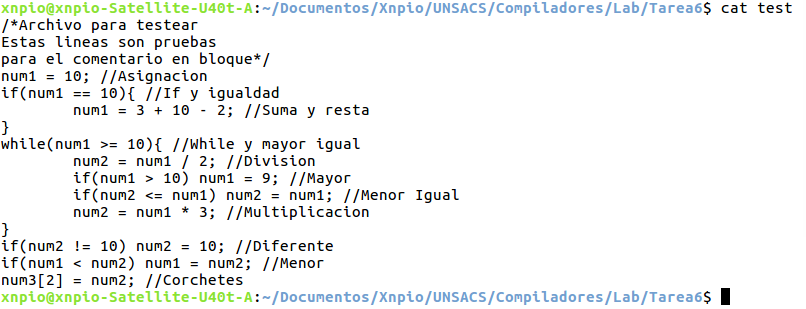
\includegraphics[scale = 0.5]{1.png}
 \caption{Archivo de prueba}
\end{figure}

\begin{figure}[H]
 \centering
 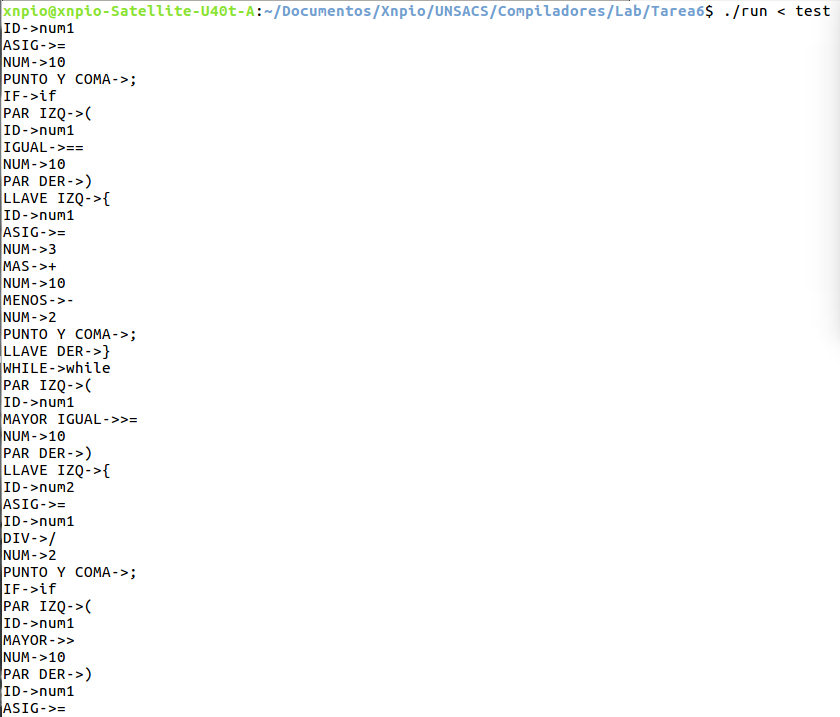
\includegraphics[scale = 0.5]{2.png}
\end{figure}
\begin{figure}[H]
 \centering
 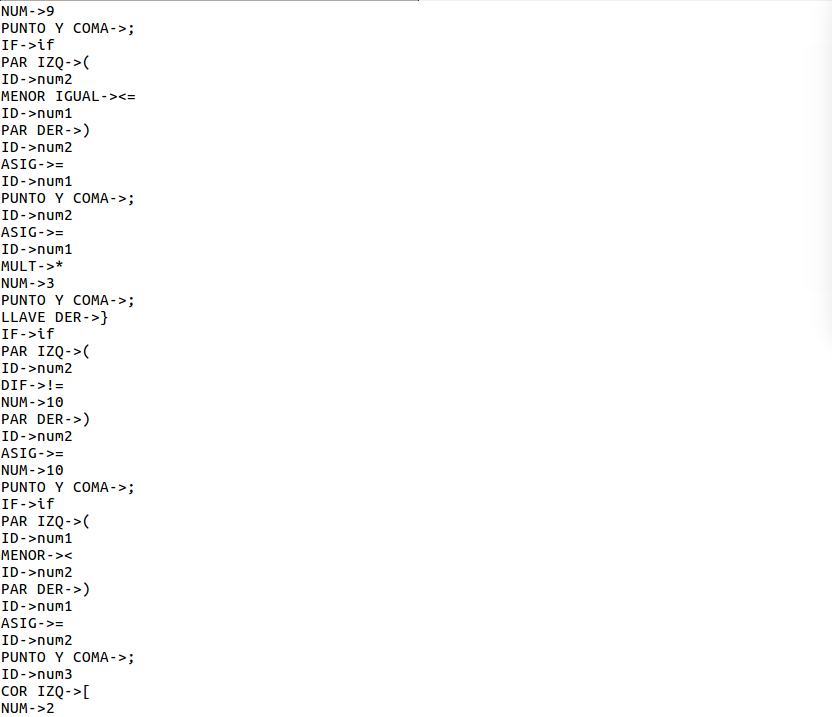
\includegraphics[scale = 0.5]{3.png}
\end{figure}
\begin{figure}[H]
 \centering
 
\includegraphics[scale = 0.5]{4.png}
 \caption{Resultados}
\end{figure}


\end{document}

